\documentclass[aspectratio=169, xcolor=table]{beamer}

% --- Carrega o Arquivo de Estilo Personalizado ---
\usepackage{cba2026}

% customization of the footline
\makeatletter
\setbeamertemplate{footline}
{
  \leavevmode%
  \hbox{%
  \begin{beamercolorbox}[wd=.333333\paperwidth,ht=2.25ex,dp=1ex,center]{author in head/foot}%
    \usebeamerfont{author in head/foot}
    Thiago Paula (UnB)
  \end{beamercolorbox}%
  \begin{beamercolorbox}[wd=.333333\paperwidth,ht=2.25ex,dp=1ex,center]{title in head/foot}%
    \usebeamerfont{title in head/foot}
    EADRC for Parkinson Tremor
  \end{beamercolorbox}%
  \begin{beamercolorbox}[wd=.333333\paperwidth,ht=2.25ex,dp=1ex,center]{date in head/foot}%
    \usebeamerfont{date in head/foot}
    XXVI CBA -- 9 de outubro de 2026
    \hspace*{2em}
    \insertframenumber{} / \inserttotalframenumber\hspace*{2ex}
  \end{beamercolorbox}}%
  \vskip0pt%
}
\makeatother


% --- Loads user-defined packages ---
\usepackage{csquotes}
\usepackage{bm}
\usepackage{multirow}
\usepackage{tabularx}
\usepackage{adjustbox}
\usepackage{appendixnumberbeamer}

% --- Reuses the paper's figures and TikZ styles (spring, damper, etc.) ---
\graphicspath{{logos/}{figures/}{../cba-2026-paper/}}
% Useful libs (TiKz and Dvipsnames packages are assumed loaded)
\usetikzlibrary{
    shapes, 
    positioning, 
    decorations.pathmorphing, 
    decorations.markings,
    patterns,
    calc,
}

% Colors
\definecolor{startstop}{HTML}{FF3867}
\definecolor{io}{HTML}{2E8B57}
\definecolor{process}{HTML}{1CA1DA}
\definecolor{decision}{HTML}{D8C303}

% Spring and damper
\tikzstyle{spring}=[
    decorate, 
    decoration={
        coil,
        segment length = 1mm,
        amplitude = 1mm,
    }
]
\tikzstyle{damper}=[
    decoration={
    markings,  
      mark connection node=dmp,
      mark=at position 0.5 with 
      {
        \node (dmp) [thick,inner sep=0pt,transform shape,rotate=-90,minimum width=5pt,minimum height=1pt,draw=none] {};
        \draw [thick] ($(dmp.north east)+(1pt,0)$) -- (dmp.south east) -- (dmp.south west) -- ($(dmp.north west)+(1pt,0)$);
        \draw [thick] ($(dmp.north)+(0,-3pt)$) -- ($(dmp.north)+(0,2pt)$);
      }
    }, 
    decorate
]

% Flowchart blocks
\tikzstyle{startstop} = [
    rectangle, 
    rounded corners, 
    minimum width=2cm, 
    minimum height=1cm,
    text centered, 
    draw=black, 
    fill=startstop!50,
]

\tikzstyle{process} = [
    rectangle, 
    minimum width=2cm, 
    minimum height=1cm, 
    text centered, 
    draw=black, 
    trapezium stretches=true,
    fill=process!50,
]
\tikzstyle{io} = [
    trapezium, 
    trapezium left angle=70, 
    trapezium right angle=110, 
    minimum width=2cm, 
    minimum height=1cm, 
    text centered, 
    draw=black, 
    trapezium stretches=true,
    fill=io!30,
]
\tikzstyle{decision} = [
    diamond, 
    minimum width=1cm, 
    minimum height=1cm, 
    text centered, 
    draw=black, 
    fill=decision!50,
]

% Control diagram blocks
\tikzstyle{sum} = [
    draw,
    circle,
    minimum size=0.6cm,
    fill=Rhodamine!70,
]
% When using a sum shape, lines must be drawn and +- sign indicated
% \draw 
% (sum.north east) -- (sum.south west)
% (sum.north west) -- (sum.south east);
% \node[left=-1pt] at (sum.center){\tiny $+$};
% \node[below] at (sum.center){\tiny $-$};
\tikzstyle{controller} = [
    draw,
    fill=Peach!90,
    minimum width=1.2cm,
    minimum height=0.9cm,
]
\tikzstyle{system} = [
    draw,
    fill=Peach!90,
    minimum width=1.2cm,
    minimum height=0.9cm,
]
\tikzstyle{sensor} = [
    draw,
    fill=Goldenrod!80,
    minimum width=1.2cm,
    minimum height=0.9cm,
]
\usetikzlibrary{fit}

% Overlay-aware TikZ elements: `visible on=<2->` hides an element (keeping its space) outside
% those slides; \tikzset{visible on/.style={}} shows everything at once
\tikzset{
  invisible/.style = {opacity = 0, text opacity = 0},
  visible on/.style = {alt = {#1{}{invisible}}},
  alt/.code args = {<#1>#2#3}{\alt<#1>{\pgfkeysalso{#2}}{\pgfkeysalso{#3}}},
}

% Upper limb schematic from the paper, typeset at the paper's column width so that
% its annotations stay aligned with the skeleton picture, and scaled afterwards
\newcommand{\upperlimbschematic}{%
  {\setlength{\linewidth}{251.80688pt}%
  \begin{tikzpicture}[scale=1.066, > = latex]

    % Invisible vertical padding
    \draw [white] (0,2.75) circle (1);

    \node [opacity=0.25] at (0,0) {
        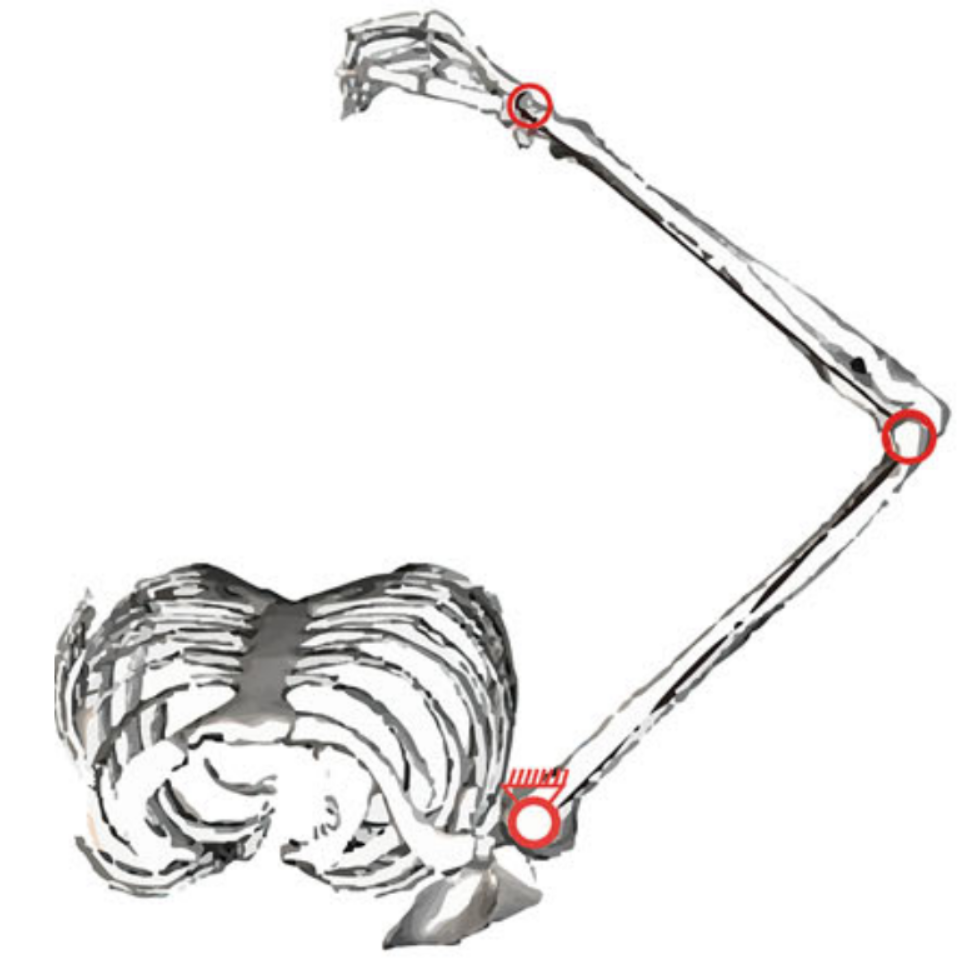
\includegraphics[width=0.8\linewidth]
        {figures/skeleton.png}
    };
    
    \coordinate (shoulder) at (0.37, -2.37);
    \path (shoulder) +(45.9:3.725) coordinate (elbow);
    \path (elbow) +(138.7:3.47) coordinate (wrist);
    \path (wrist) +(138.7:0.9) coordinate (knuckle);
    
    % test coordinates alignments (debug only)
    % \draw [cyan, fill=cyan, opacity=0.2, thick, dashed] (shoulder) circle (0.3);
    % \draw [cyan, fill=cyan, opacity=0.2, thick, dashed] (elbow) circle (0.3);
    % \draw [cyan, fill=cyan, opacity=0.2, thick, dashed] (wrist) circle (0.3);
    % \draw [cyan, fill=cyan, opacity=0.2, thick, dashed] (knuckle) circle (0.3);

    % Arm annotations
    \draw [|-|, opacity=0.5] (shoulder) ++ (-45:0.5) --++ (45.9:3.725)
        node [midway, fill=white, opacity=1.0, inner sep=0.2] {$l_1$};
    \draw [thick, orange, fill=orange, opacity=0.5]
        (shoulder) ++ (0.2, 0) 
        --++ (0.7, 0) node [right, black, opacity=1.0] {$\theta_1$}
        arc (0:45.9:0.7) -- cycle;
    \draw [thick, <->] (shoulder) ++ (0.5, 0) arc (0:90:0.5) 
        node [midway, above, xshift=0.4cm, yshift=-0.1cm] {$I_1, \tau_1$};

    % Forearm annotations
    \draw [|-|, opacity=0.5] (elbow) ++ (45:0.55) --++ (142:3.5)
        node [midway, fill=white, opacity=1.0, inner sep=0.2] {$l_2$};
    \draw [thick, orange, fill=orange, opacity=0.5]
        (elbow) ++ (42:0.35) 
        --++ (45:0.7) arc (45:142:0.7) 
        node [midway, above, black, opacity=1.0] {$\theta_2$}
        -- cycle;
    \draw [thick, <->] (elbow) ++ (175:0.3)
        arc (180:90:0.5) node [below, xshift=0.2cm, yshift=-0.2cm] {$I_2, \tau_2\quad$};

    % Wrist annotations
    \draw [|-|, opacity=0.5] (wrist) ++ (45:0.3) --++ (138:0.9)
        node [midway, fill=white, opacity=1.0, inner sep=0.2] {$l_3$};
    \draw [thick, orange, fill=orange, opacity=0.5]
        (wrist)
        --++ (142:0.7) 
        arc (142:135:0.7) 
        node [midway, left, black, opacity=1.0] {$\theta_3$} 
        -- cycle;
    \draw [thick, <->] (wrist) node [xshift=0.1cm, yshift=0cm] {$I_3, \tau_3$} ++ (100:0.3)
        arc (100:170:0.4) ;

    % Stiffness and damping
    
    %% Shoulder
    \draw [spring] (shoulder) ++ (97:1.05) arc (97:45:1.05);
    \draw [postaction={damper}] (shoulder) ++ (98:1.3) arc (98:45:1.3)
        node [midway, above, sloped, yshift=0.1cm] {$k_1$, $c_1$};
        
    %% Elbow            
    \draw [spring] (elbow) ++ (-135:0.5) arc (-135:-225:0.5);
    \draw [postaction={damper}] (elbow) ++ (-135:0.8) 
    arc (-135:-225:0.8)
    node [midway, above, sloped, yshift=0.1cm] {$k_2$, $c_2$};
    %% Biceps
    \draw [spring] (elbow) ++ (-135:3.7) arc (-135:-280:2);
    \draw [postaction={damper}] (elbow) ++ (-135:4) 
        arc (-135:-270:2.3)
        node [midway, above, sloped, yshift=0.1cm] {$k_3$, $c_3$};
    %% Wrist
    \draw [spring] (wrist) ++ (175:0.5) arc (175:317:0.5);
    \draw [postaction={damper}] (wrist) ++ (176:0.8) 
        arc (176:317:0.8)
        node [midway, below, sloped] {$k_4$, $c_4$}; 
    
\end{tikzpicture}\unskip}%
}

% --- Arquivo de Referências (the paper's bibliography) ---
\addbibresource{../cba-2026-paper/references/active_disturbance_rejection_control_theory.bib}
\addbibresource{../cba-2026-paper/references/c1_tremor_characterization_reviews.bib}
\addbibresource{../cba-2026-paper/references/c2_tremor_suppression_reviews.bib}
\addbibresource{../cba-2026-paper/references/c3_passive_control_strategies.bib}
\addbibresource{../cba-2026-paper/references/c4_active_control_strategies.bib}
\addbibresource{../cba-2026-paper/references/metrics.bib}
\addbibresource{references.bib}

% Sorted numbers in multiple citations, e.g. [1, 4] instead of [4, 1]
\ExecuteBibliographyOptions{sortcites=true}
% Acronyms such as DOI and ISBN in plain capitals, since the sans serif font has no small caps
\renewrobustcmd*{\mkbibacro}[1]{#1}
\renewcommand*{\bibfont}{\scriptsize}


 
% --- Dados da Apresentação ---
\title[EADRC for Parkinson Tremor]{
  EADRC for Parkinson Tremor Suppression in Wrist Considering Upper Limb Dynamics\\
  % \rule{\textwidth}{.5pt}\\
  % {\small Supressão de tremor de Parkinson no punho via EADRC considerando dinâmicas do membro superior}
}
\subtitle{Supressão de tremor de Parkinson no punho via EADRC considerando dinâmicas do membro superior}
\author[Paula, Thiago et al.]{
  \texorpdfstring{%
    \underline{Thiago T. de Paula}, Matheus T. de Sousa,\\
    José O. A. L. Filho, Marcela R. Machado
  }{%
    Thiago T. de Paula, Matheus T. de Sousa,
    José O. A. L. Filho, Marcela R. Machado
  }
}
\institute[UnB]{Universidade de Brasília}
\date{Outubro, 2026}

% =========================================================================
% CONTEÚDO DO DOCUMENTO
% =========================================================================
\begin{document}

% 1. Capa
\begin{frame}[plain]
  \titlepage
\end{frame}

% 2. Sumário
% \begin{frame}{Sumário}
%   \tableofcontents
% \end{frame}

\section{Introdução}

\begin{frame}{Doença de Parkinson e tremor}
  \begin{columns}[T]
    \begin{column}{0.48\textwidth}
      \begin{block}{A doença}
        \begin{itemize}
          \item Distúrbio neurodegenerativo crônico e progressivo: perda de neurônios dopaminérgicos na substância negra \cite{Meng:2022,Fujikawa:2023}.
          \item Manifestações motoras: bradicinesia, rigidez, instabilidade postural e \alert{tremor de repouso} \cite{Botzel:2014}.
        \end{itemize}
      \end{block}
    \end{column}
    \begin{column}{0.48\textwidth}
      \begin{block}{Tratamentos convencionais}
        \begin{itemize}
          \item Farmacológico: primeira linha, mas parte dos pacientes não responde, e o uso prolongado perde eficácia e causa efeitos colaterais \cite{Fujikawa:2023,Lora-Millan:2021,Meng:2022}.
          \item Cirúrgico: invasivo e com riscos \cite{Botzel:2014,Fujikawa:2023}.
        \end{itemize}
      \end{block}
    \end{column}
  \end{columns}

  \vspace{0.4cm}
  \begin{exampleblock}{Órteses com controle ativo}
    Alternativa eficaz e não invasiva \cite{Lora-Millan:2021,Meng:2022}, particularmente popular para a supressão do tremor de punho.
  \end{exampleblock}
\end{frame}

\begin{frame}{Supressão ativa do tremor de punho}
  \centering
  \small
\begin{tabularx}{\textwidth}{
    l
    >{\raggedright\arraybackslash\hsize=1.2\hsize}X
    >{\raggedright\arraybackslash\hsize=0.8\hsize}X
}
    \toprule
    Trabalho & Controle e planta & Estimação \\
    \midrule
    \textcite{Gallego:2013} & PI (neuroprótese), punho com 1 GdL & CDF + WFLC + KF \\\midrule
    \textcite{Copur:2019} & Controle repetitivo (estimulação elétrica), 1 GdL & Passa-altas de fase zero \\\midrule
    \textcite{Lekshmi:2019} & PID com ganhos por algoritmo genético, braço com 4 GdL (punho com 1 GdL) & Movimento voluntário ausente \\\midrule
    \textcite{Zamanian:2019} & Filtro \textit{notch} adaptativo, punho com 1 GdL & Frequência do tremor via AFE \\\midrule
    \textcite{Qi:2024} & ADRC, punho com 1 GdL & Movimento voluntário via EBMFLC \\
    \bottomrule
\end{tabularx}


  \vspace{0.3cm}
  \begin{alertblock}{Lacuna}
    Tremores de ombro e cotovelo afetam significativamente o movimento do punho,
    mas a maioria das abordagens usa modelos de uma única articulação, desprezando o acoplamento entre elas.
  \end{alertblock}
\end{frame}

\begin{frame}{Proposta deste trabalho}
  \begin{itemize}
    \setlength{\itemsep}{0.25cm}
    \item \textbf{Controle:} rejeição ativa de perturbações baseada em erro (EADRC), robusta a perturbações externas e incertezas de modelo \cite{Guo:2016}.
    \item \textbf{Plataforma de teste:} modelo linear do membro superior com 3 graus de liberdade (GdL) \cite{Gebai:2017,Gebai:2018}, que captura o acoplamento ombro--cotovelo--punho.
    \item \textbf{Estimação do movimento voluntário}, em duas variantes:
      \begin{itemize}
        \item EADRC+EBMFLC, com o combinador linear de Fourier de \textcite{Qi:2024};
        \item EADRC+ZPLP, com filtragem passa-baixas de fase zero (ZPLP).
      \end{itemize}
    \item \textbf{Comparação} com dois PIDs: IMC-PID (\textit{Internal Model Control}) e DE-PID (evolução diferencial com conhecimento perfeito do movimento voluntário).
    \item \textbf{Robustez:} 100 simulações de Monte Carlo dos parâmetros físicos e teste de Wilcoxon pareado.
  \end{itemize}
\end{frame}

\section{Fundamentação Teórica}

\begin{frame}{Modelo do membro superior}
  \begin{columns}[c]
    \begin{column}{0.40\textwidth}
      \centering
      \resizebox{!}{0.68\textheight}{\upperlimbschematic}

      {\scriptsize Adaptado de \textcite{Albuquerque:2025}.}
    \end{column}
    \begin{column}{0.58\textwidth}
      \begin{itemize}
        \item Modelo planar com 3 GdL: ombro ($\theta_1$), cotovelo ($\theta_2$) e punho ($\theta_3$) \cite{Gebai:2018}.
        \item Músculos e tendões como molas e amortecedores equivalentes; $k_3$ representa o acoplamento pelo bíceps.
      \end{itemize}
      \begin{equation*}
        \mathbf{J}\ddot{\bm{\theta}} + \mathbf{C}\dot{\bm{\theta}} + \mathbf{K}\bm{\theta} = \bm{\tau},
        \,\,
        \mathbf{K} =
        \begin{bmatrix}
          k_1 + k_3 & k_3       & 0   \\
          k_3       & k_2 + k_3 & 0   \\
          0         & 0         & k_4
        \end{bmatrix}
      \end{equation*}
      \begin{itemize}
        \item $\mathbf{C}$ tem a estrutura de $\mathbf{K}$, com $c_i \propto k_i$; $\mathbf{J}$ é cheia e acopla as três articulações.
        \item Linearização adequada se os parâmetros variam pouco no tempo \cite{Gebai:2020}.
      \end{itemize}
    \end{column}
  \end{columns}
\end{frame}

\begin{frame}{Torques aplicados e representação em espaço de estados}
  \begin{columns}[T]
    \begin{column}{0.5\textwidth}
      \begin{block}{Torque em um paciente com DP \cite{Qi:2024}}
        \vspace{-0.3cm}
        \begin{equation*}
          \bm{\tau} = \underbrace{\bm{\tau}_i}_{\text{patológico}} + \underbrace{\bm{\tau}_v}_{\text{voluntário}}
        \end{equation*}
      \end{block}
      \begin{itemize}
        \item A potência do tremor concentra-se em torno de uma frequência central \cite{Deuschl:2022}; usualmente, até 3 harmônicos \cite{Zamanian:2019,Albuquerque:2025}.
        \item O acoplamento já torna a dinâmica do punho multimodal: um harmônico por articulação.
      \end{itemize}
    \end{column}
    \begin{column}{0.46\textwidth}
      \begin{block}{Tremor}
        \begin{equation*}
          \bm{\tau}_i =
          \begin{bmatrix}
            A_1\sin(2\pi f_1 t) \\
            A_2\sin(2\pi f_2 t) \\
            A_3\sin(2\pi f_3 t)
          \end{bmatrix}
        \end{equation*}
        \centering
        \small
        $A_i = 1$~N$\cdot$m;\quad $f_1\ f_2\ f_3 = 3{,}59\ 5{,}30\ 14{,}35$~Hz
      \end{block}
      \begin{block}{Espaço de estados, $\mathbf{x} = [\bm{\theta}^\top\ \dot{\bm{\theta}}^\top]^\top$}
        \vspace{-0.3cm}
        \begin{align*}
          \dot{\mathbf{x}} &= \mathbf{A}\mathbf{x} + \mathbf{B}\bm{\tau}, \qquad
          \mathbf{y} = \mathbf{C}_\text{ss}\mathbf{x} \\[1mm]
          \mathbf{A} &=
          \begin{bmatrix}
            \mathbf{0} & \mathbf{I} \\
            -\mathbf{J}^{-1}\mathbf{K} & -\mathbf{J}^{-1}\mathbf{C}
          \end{bmatrix},
          \quad
          \mathbf{B} =
          \begin{bmatrix}
            \mathbf{0} \\
            \mathbf{J}^{-1}
          \end{bmatrix} \\[1mm]
          \mathbf{C}_\text{ss} &=
          \begin{bmatrix}
            \mathbf{I} & \mathbf{0}
          \end{bmatrix}
        \end{align*}
      \end{block}
    \end{column}
  \end{columns}
\end{frame}

\begin{frame}{Controle por rejeição ativa de perturbações baseado em erro}
  \begin{columns}[T]
    \begin{column}{0.48\textwidth}
      \begin{itemize}
        \item ADRC: estima e rejeita, em tempo real, a \alert{perturbação total}, isto é, incertezas internas e perturbações externas \cite{Guo:2016}:
          \begin{equation*}
            y^{(n)} = f(y, \dot{y}, \dots, y^{(n-1)}, t) + b_0 u.
          \end{equation*}
        \item EADRC: mesma estrutura no erro de rastreamento $e = r - y$, de implementação mais simples \cite{Madonski:2019}:
          \begin{equation*}
            e^{(n)} = f_e - b_0 u,
            \qquad
            f_e = r^{(n)} - f(\cdot).
          \end{equation*}
      \end{itemize}
    \end{column}
    \begin{column}{0.48\textwidth}
      ESO, com $z_i = e^{(i-1)}$ ($i \leq n$) e $z_{n+1} = f_e$:
      \begin{equation*}
        \begin{cases}
          \dot{\hat{z}}_i = \hat{z}_{i+1} + \beta_i (e - \hat{z}_1), \quad i < n \\
          \dot{\hat{z}}_n = \hat{z}_{n+1} + \beta_n (e - \hat{z}_1) - b_0 u \\
          \dot{\hat{z}}_{n+1} = \beta_{n+1} (e - \hat{z}_1)
        \end{cases}
      \end{equation*}
      Lei de controle e dinâmica resultante do erro:
      \begin{align*}
        u &= \tfrac{1}{b_0}\big(\textstyle\sum_{i=1}^{n} \kappa_i \hat{z}_i + \hat{z}_{n+1}\big) \\
        \implies\ e^{(n)} &\approx -\textstyle\sum_{i=1}^{n} \kappa_i e^{(i-1)}
      \end{align*}
    \end{column}
  \end{columns}

  \begin{alertblock}{Cuidado}
    \small
    Usualmente, limita-se a magnitude ou a taxa do sinal de controle 
    para evitar instabilidade do observador\cite{Herbst:2025}.
  \end{alertblock}
\end{frame}

\section{Metodologia}

\begin{frame}{EADRC aplicado ao punho}
  \begin{columns}[T]
    \begin{column}{0.48\textwidth}
      \begin{itemize}[<+->]
        \item Sistema linear: o ângulo do punho tem parcelas voluntária e involuntária,
          \begin{equation*}
            \theta_3 = \theta_{v_3} + \theta_{i_3}.
          \end{equation*}
        \item Torque de controle apenas no punho, $\mathbf{u} = [0\ \ 0\ \ u_3]^\top$:
          \begin{equation*}
            \ddot{\theta}_3 = b_0 u_3 + \zeta(\bm{\tau}, \bm{\theta}, \dot{\bm{\theta}}),
            \quad
            b_0 = \left[\mathbf{J}^{-1}\right]_{33}.
          \end{equation*}
        \item $\zeta$ inclui o acoplamento com ombro e cotovelo, tratado como parte da perturbação total ($n = 2$).
      \end{itemize}
    \end{column}
    \begin{column}{0.48\textwidth}
      \begin{itemize}[<+->]
        \item 
        Erro ideal, que vai a zero quando $u_3$ compensa $\tau_{i_3}$:
          \begin{equation*}
            e_3 = \bm{\theta_{v_3}} - \theta_3 = -\theta_{i_3}.
          \end{equation*}
        Na prática, $\theta_{v_3}$ é desconhecido e estimado,
          \begin{equation*}
            \hat{e}_3 = \bm{\hat{\theta}_{v_3}} - \theta_3,
          \end{equation*}
        \alert{e a qualidade da estimativa limita a supressão alcançável.}
      \end{itemize}
    \end{column}
  \end{columns}
\end{frame}

\begin{frame}{Malha de controle e estimadores de movimento voluntário}
  \centering
  % Closed loop of the error-based ADRC applied to the wrist joint
% (needs TikZ libraries positioning, calc and fit, and the CBA colors from cba2026.sty)
\begin{tikzpicture}[
    > = latex,
    font = \small,
    block/.style = {
        draw,
        thick,
        rounded corners = 2pt,
        align = center,
        minimum height = 0.95cm,
        inner sep = 4pt,
    },
    eadrc/.style = {block, draw = CBAPurple, fill = CBALightPurple, minimum width = 2.2cm},
    plant/.style = {block, draw = CBAOrange, fill = CBALightOrange},
    estimator/.style = {block, draw = CBAPetrol, fill = CBALightPetrol},
    junction/.style = {draw, thick, circle, minimum size = 0.45cm, inner sep = 0pt},
]
    % Blocks
    \node [junction] (sum) {};
    \node [eadrc, right = 1.2cm of sum] (eso) {ESO\\baseado em erro};
    \node [eadrc, right = 1.6cm of eso] (law) {Lei de\\controle};
    \node [plant, right = 1.6cm of law] (plant) {Membro superior\\(3 GdL)};
    \node [estimator] (estimator) at ($(eso)!0.5!(law) + (0, -1.55)$)
        {Estimador de movimento voluntário\\(ZPLP ou EBMFLC)};

    % EADRC frame
    \node [
        draw = CBAPurple,
        dashed,
        rounded corners = 4pt,
        inner xsep = 0.25cm,
        inner ysep = 0.2cm,
        fit = (eso) (law),
        label = {[CBAPurple, font = \small\bfseries]north:EADRC},
    ] (eadrc frame) {};

    % Auxiliary coordinates
    \coordinate (u branch) at ($(law.east)!0.45!(plant.west)$);
    \coordinate (y branch) at ($(plant.east) + (0.45, 0)$);
    \coordinate (output) at ($(plant.east) + (1.3, 0)$);

    % Forward path
    \draw [->, thick] (sum) -- (eso) node [midway, above] {$\hat{e}_3$};
    \draw [->, thick] (eso) -- (law) node [midway, above] {$\hat{\bm{z}}$};
    \draw [->, thick] (law) -- (plant) node [pos = 0.45, above] {$u_3$};
    \draw [->, thick] (plant) -- (output) node [at end, above left] {$\theta_3$};

    % Control signal fed back to the observer
    \fill (u branch) circle (1.5pt);
    \draw [->, thick] (u branch) |- ($(eadrc frame.south) + (0, -0.2)$) -| (eso.south);

    % Torques acting on the upper limb
    \draw [<-, thick] (plant.north) -- ++(0, 0.6) node [above] {$\bm{\tau}_i + \bm{\tau}_v$};

    % Measured wrist angle fed back through the estimator (+) and directly (-)
    \fill (y branch) circle (1.5pt);
    \draw [->, thick] (y branch) |- (estimator.east);
    \draw [->, thick] (estimator.west) -| (sum.south)
        node [pos = 0.25, above] {$\hat{\theta}_{v_3}$}
        node [at end, below right = -1pt] {\scriptsize $+$};
    \draw [->, thick] (y branch) |- ($(estimator.south) + (0, -0.45)$) -| ($(sum.west) + (-0.6, 0)$)
        -- (sum.west) node [at end, above left = -1pt] {\scriptsize $-$};
\end{tikzpicture}


  \pause
  \vspace{0.3cm}
  \begin{columns}[T]
    \begin{column}{0.48\textwidth}
      \begin{exampleblock}{ZPLP}
        \small
        Butterworth passa-baixas de 1ª ordem, corte em 5 Hz, filtrado nos dois sentidos (fase zero) sobre as amostras disponíveis até o instante atual.
      \end{exampleblock}
    \end{column}
    \begin{column}{0.48\textwidth}
      \pause
      \begin{exampleblock}{EBMFLC \cite{Qi:2024}}
        \small
        Combinação linear adaptativa de 100 senoides entre 0 e 12 Hz; a parcela de 0 a 4 Hz é tomada como movimento voluntário.
      \end{exampleblock}
    \end{column}
  \end{columns}
\end{frame}

\begin{frame}{Simulações de Monte Carlo}
  \begin{columns}[T]
    \small
    \begin{column}{0.58\textwidth}
      \begin{itemize}
        \item Runge-Kutta de 4ª ordem, $t \in [0, 6]$~s, passo de 1~ms.
        \item 100 execuções por controlador: a primeira com o modelo nominal \cite{Gebai:2018}, as demais com rigidezes reamostradas ($c_i \propto k_i$ acompanha).
        \item Mesma semente aleatória para todos os controladores: comparação pareada.
      \end{itemize}
      %
      \pause
      \vspace{0.2cm}
      \centering
      \footnotesize
\begin{tabular}{l c c c c}
    \toprule
    Rigidez [N$\cdot$m/rad] & Mín. & Nominal & Máx. & Variação \\
    \midrule
    $k_1$ (ombro)    & 150 & 180 & 210 & $\pm16\%$ \\
    $k_2$ (cotovelo) & 50  & 70  & 90  & $\pm28\%$ \\
    $k_3$ (bíceps)   & 30  & 40  & 50  & $\pm25\%$ \\
    $k_4$ (punho)    & 5   & 10  & 15  & $\pm50\%$ \\
    \bottomrule
\end{tabular}

    \end{column}

    \pause
    \begin{column}{0.40\textwidth}
      \begin{itemize}
        \item Cenários: \alert{repouso} ($\bm{\tau}_v = \mathbf{0}$) e \alert{movimento} ($\bm{\tau}_v$ senoidal).
      \end{itemize}
      \centering
      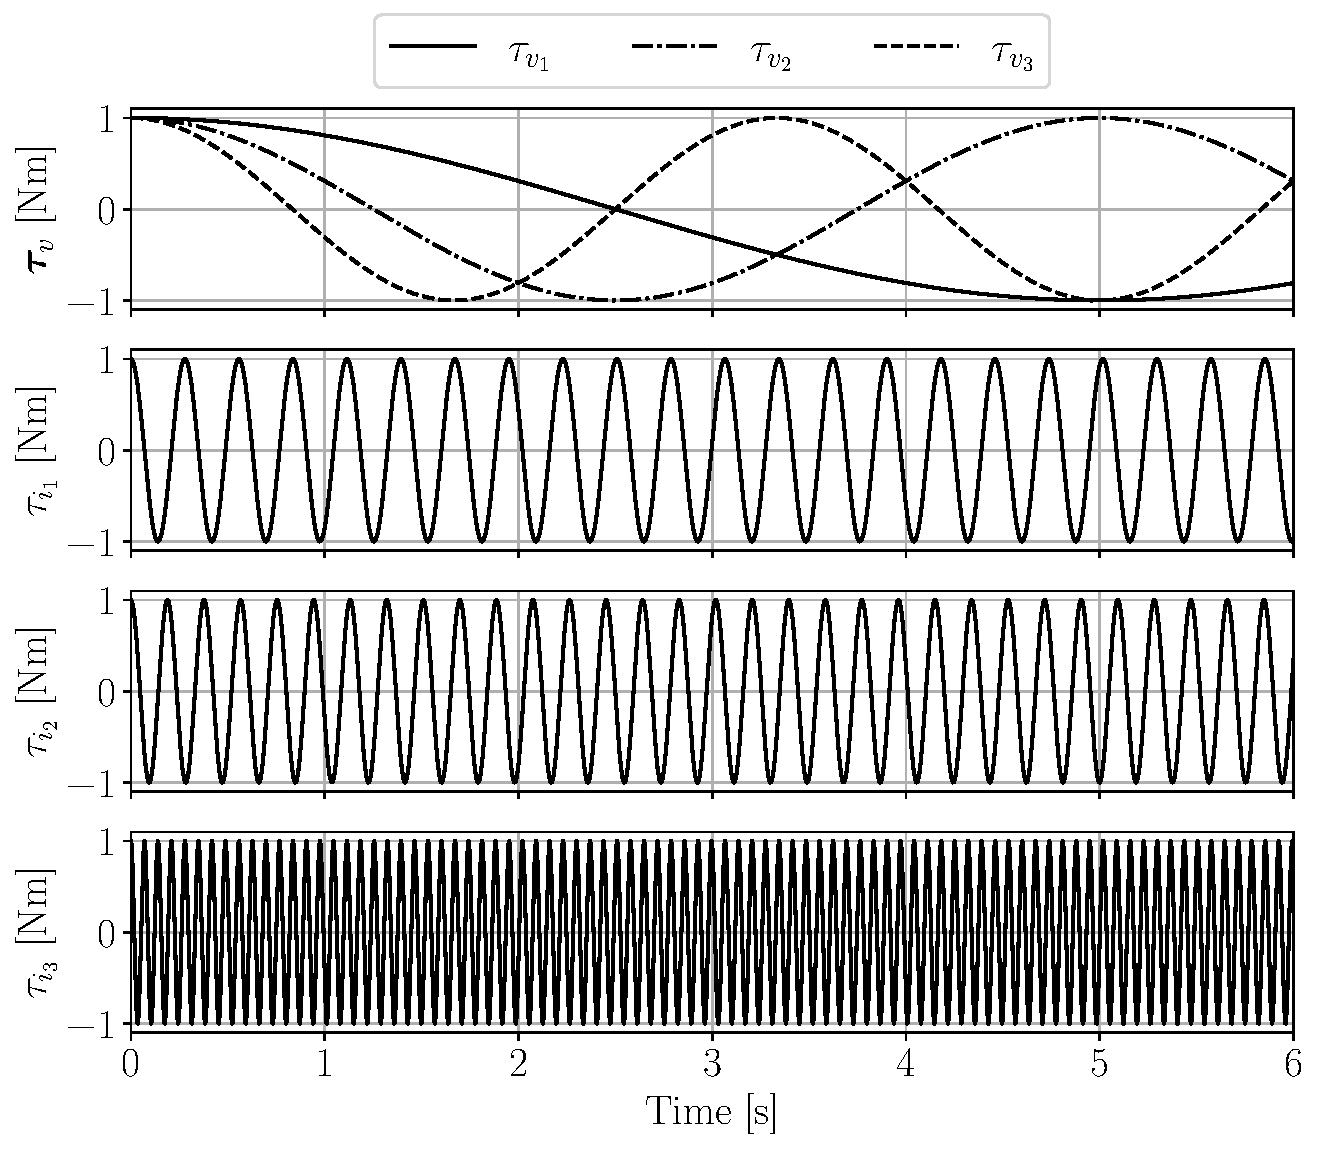
\includegraphics[width=\linewidth]{figures/plots/uncontrolled_amplitude_1.0/torque_profiles_uncontrolled_amplitude_1.0.pdf}

      {\scriptsize Torques voluntários (movimento) e de tremor.}
    \end{column}
  \end{columns}
\end{frame}

\begin{frame}{Controladores e métricas de desempenho}
  \centering
  \footnotesize
\begin{tabularx}{\textwidth}{l >{\raggedright\arraybackslash}X l}
    \toprule
    Controlador & Parâmetros & Sintonia (modelo nominal) \\
    \midrule
    EADRC+ZPLP &
        $\omega_c = 10$, $\omega_o = 100$; Butterworth de 1ª ordem, corte em 5 Hz &
        Experimental, $\omega_o = 10\,\omega_c$ \\
    EADRC+EBMFLC &
        $\omega_c = 20$, $\omega_o = 80$; $n = 100$, $\mu = 0{,}005$, $T_p = 0{,}59$~s, $\alpha = 0{,}02$ &
        Experimental, $\omega_o = 4\,\omega_c$ \\
    IMC-PID &
        $K_p = 1{,}235$, $K_i = 1234{,}660$, $K_d = 0{,}506$ &
        IMC \cite{Rivera:1986}, punho isolado, $\lambda = 0{,}4\,\tau$ \\
    DE-PID &
        $K_p = 1{,}721$, $K_i = 15{,}059$, $K_d = 3{,}239$ &
        Evolução diferencial, $\theta_{v_3}$ conhecido \\
    \bottomrule
\end{tabularx}


  \pause
  \vspace{0.4cm}
  \begin{columns}[T]
    \begin{column}{0.48\textwidth}
      \begin{block}{Métricas}
        \small
        \begin{itemize}
          \item Resposta do punho: TPSR \cite{Qi:2024}, IAE \cite{Skogestad:2003}, $R^2$ \cite{Glantz:1990} e entropia \cite{Lathi:2018}.
          \item Sinal de controle: variação total (TV) \cite{Skogestad:2003} e potência \cite{Lathi:2018}.
        \end{itemize}
      \end{block}
    \end{column}
    \begin{column}{0.48\textwidth}
      \pause
      \begin{block}{Análise estatística}
        \small
        \begin{itemize}
          \item EADRC+ZPLP contra cada controlador: teste de Wilcoxon pareado \cite{Conover:1980}, com correlação bisserial de postos $r$.
          \item Correção de Holm-Bonferroni nas seis métricas; significância em $0{,}05$.
        \end{itemize}
      \end{block}
    \end{column}
  \end{columns}
\end{frame}

\section{Resultados e Discussão}

\begin{frame}{Métricas médias em 100 execuções}
  \centering
  \begin{adjustbox}{max width=\textwidth}
\scriptsize
\setlength{\tabcolsep}{4pt}
\renewcommand{\arraystretch}{1.15}
% Mean followed by its standard deviation, the latter in a slightly smaller font (7 pt vs. 8 pt)
\newcommand{\meanstd}[2]{#1\,{\fontsize{7}{8}\selectfont$\pm$\,#2}}
\begin{tabular}{>{\cellcolor{white}}c l c c c c c c}
    \toprule
    & &
    \multicolumn{4}{c}{Resposta do punho} &
    \multicolumn{2}{c}{Sinal de controle} \\
    \cmidrule(lr){3-6} \cmidrule(lr){7-8}
    & Controlador &
    TPSR $\uparrow$ & $R^2$ $\uparrow$ & Entropia $\downarrow$ & IAE $\downarrow$ & Potência $\downarrow$ & TV $\downarrow$ \\
    & &
    [\%] & [---] & [bits] & [rad$\cdot$s] & [(N$\cdot$m)$^2$] & [N$\cdot$m$\cdot$s] \\
    \midrule
    & EADRC+EBMFLC & \meanstd{45,92}{54,00} & \meanstd{0,41}{0,15} & \meanstd{5,18}{0,16} & \meanstd{0,83}{0,28} & \meanstd{0,50}{0,26} & \meanstd{307,44}{89,98} \\
    \rowcolor{CBALightPurple}
    & EADRC+ZPLP & \meanstd{57,49}{35,50} & \meanstd{0,46}{0,20} & \meanstd{5,17}{0,19} & \meanstd{0,76}{0,20} & \meanstd{0,34}{0,12} & \meanstd{263,51}{47,82} \\
    & DE-PID & \meanstd{99,90}{0,10} & \meanstd{1,00}{0,00} & \meanstd{4,85}{0,10} & \meanstd{0,03}{0,01} & \meanstd{0,98}{0,38} & \meanstd{877,68}{198,91} \\
    \multirow{-4}{*}{\rotatebox{90}{Repouso}}
    & IMC-PID & \meanstd{$-$123,32}{563,17} & \meanstd{$-$0,37}{1,85} & \meanstd{5,50}{0,31} & \meanstd{1,24}{1,03} & \meanstd{8,75}{25,33} & \meanstd{492,03}{260,60} \\
    \midrule
    & EADRC+EBMFLC & \meanstd{45,02}{54,72} & \meanstd{0,46}{0,12} & \meanstd{5,23}{0,13} & \meanstd{0,84}{0,28} & \meanstd{0,51}{0,26} & \meanstd{308,50}{89,95} \\
    \rowcolor{CBALightPurple}
    & EADRC+ZPLP & \meanstd{56,97}{35,77} & \meanstd{0,51}{0,16} & \meanstd{5,21}{0,15} & \meanstd{0,76}{0,20} & \meanstd{0,35}{0,12} & \meanstd{264,31}{47,75} \\
    & DE-PID & \meanstd{99,90}{0,10} & \meanstd{1,00}{0,00} & \meanstd{4,92}{0,09} & \meanstd{0,03}{0,01} & \meanstd{0,98}{0,38} & \meanstd{877,68}{198,91} \\
    \multirow{-4}{*}{\rotatebox{90}{Movimento}}
    & IMC-PID & \meanstd{$-$154,62}{684,56} & \meanstd{$-$0,40}{2,17} & \meanstd{5,50}{0,29} & \meanstd{1,31}{1,12} & \meanstd{10,39}{31,63} & \meanstd{511,02}{295,24} \\
    \bottomrule
\end{tabular}
\end{adjustbox}


  {\scriptsize Média $\pm$ desvio padrão; $\uparrow$ ($\downarrow$): maior (menor) é melhor.}

  \begin{itemize}[<+->]
    \small
    \item DE-PID: TPSR $\approx$ 99,9\%, mas conhece $\theta_{v_3}$ e tem TV $\approx 3{,}3\times$ a do EADRC+ZPLP.
    \item EADRC+ZPLP: maior TPSR entre os controladores realizáveis (56,97\% em movimento), com menor esforço que o EADRC+EBMFLC.
    \item IMC-PID: TPSR mediano acima de 50\%, mas oscilações crescentes em algumas execuções derrubam a média.
  \end{itemize}
\end{frame}

\begin{frame}{Análise estatística}
  \begin{columns}[c]
    \begin{column}{0.62\textwidth}
      \centering
      \scriptsize
\setlength{\tabcolsep}{4pt}
\begin{tabular}{c l cc cc cc}
    \toprule
    & & \multicolumn{6}{c}{EADRC+ZPLP vs.\ $\cdots$} \\
    \cmidrule(lr){3-8}
    & & \multicolumn{2}{c}{EADRC+EBMFLC} & \multicolumn{2}{c}{DE-PID} & \multicolumn{2}{c}{IMC-PID} \\
    \cmidrule(lr){3-4} \cmidrule(lr){5-6} \cmidrule(lr){7-8}
    & Métrica & $p$ & $r$ & $p$ & $r$ & $p$ & $r$ \\
    \midrule
    & TPSR     & $<$0,001 & +0,56 & $<$0,001 & $-$1,00 & $<$0,001 & +1,00 \\
    & $R^2$    & $<$0,001 & +0,61 & $<$0,001 & $-$1,00 & $<$0,001 & +1,00 \\
    & Entropia & $<$0,001 & $-$0,69 & $<$0,001 & +1,00 & $<$0,001 & $-$1,00 \\
    & IAE      & $<$0,001 & $-$0,67 & $<$0,001 & +1,00 & $<$0,001 & $-$1,00 \\
    & Potência & $<$0,001 & $-$1,00 & $<$0,001 & $-$1,00 & \alert{0,619} & \alert{+0,06} \\
    \multirow{-6}{*}{\rotatebox{90}{Repouso}}
    & TV       & $<$0,001 & $-$0,85 & $<$0,001 & $-$1,00 & $<$0,001 & +1,00 \\
    \midrule
    & TPSR     & $<$0,001 & +0,60 & $<$0,001 & $-$1,00 & $<$0,001 & +1,00 \\
    & $R^2$    & $<$0,001 & +0,67 & $<$0,001 & $-$1,00 & $<$0,001 & +1,00 \\
    & Entropia & $<$0,001 & $-$0,86 & $<$0,001 & +1,00 & $<$0,001 & $-$1,00 \\
    & IAE      & $<$0,001 & $-$0,69 & $<$0,001 & +1,00 & $<$0,001 & $-$1,00 \\
    & Potência & $<$0,001 & $-$1,00 & $<$0,001 & $-$1,00 & $<$0,001 & $-$0,70 \\
    \multirow{-6}{*}{\rotatebox{90}{Movimento}}
    & TV       & $<$0,001 & $-$0,86 & $<$0,001 & $-$1,00 & $<$0,001 & +1,00 \\
    \bottomrule
\end{tabular}


      \vspace{0.1cm}
      {\scriptsize $p$ corrigido por Holm-Bonferroni; $r > 0$: métrica maior com EADRC+ZPLP; em vermelho, $p \geq 0{,}05$.}
    \end{column}
    \begin{column}{0.36\textwidth}
      \small
      \begin{itemize}[<+->]
        \setlength{\itemsep}{0.2cm}
        \item \textbf{vs.\ EBMFLC:} maior supressão (TPSR, IAE) e \textbf{menor esforço} de controle (potência menor em todas as execuções); entropia equivalente em repouso.
        \item \textbf{vs.\ DE-PID:} $|r| \approx 1$ em todas as métricas: resposta melhor em todas as execuções, à custa de maior esforço em todas elas.
        \item \textbf{vs.\ IMC-PID:} supressão superior ($|r| \geq 0{,}94$ em TPSR, $R^2$ e IAE) e \textbf{menor esforço} em todas as execuções (potência e TV).
      \end{itemize}
    \end{column}
  \end{columns}
\end{frame}

\begin{frame}{Espectrogramas da resposta do punho}
  \begin{columns}[c]
    \begin{column}{0.68\textwidth}
      \centering
      \begin{minipage}{0.49\linewidth}
        \centering
        {\scriptsize Sem controle, repouso}\\
        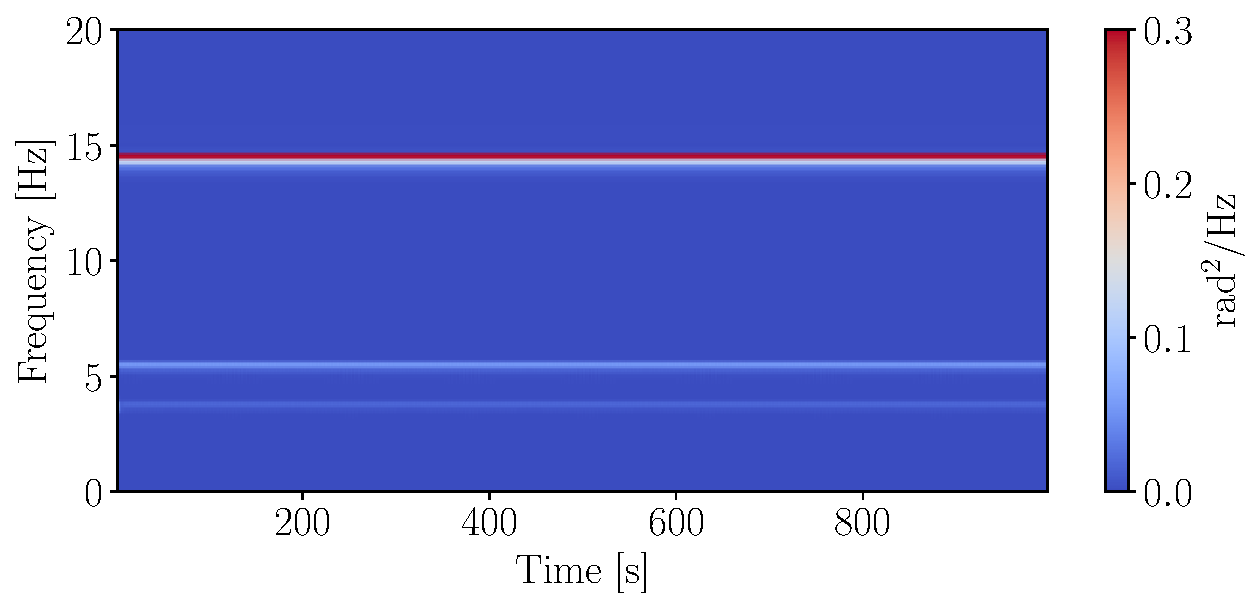
\includegraphics[width=\linewidth]{figures/plots/uncontrolled_amplitude_0.0/spectrogram_response_uncontrolled_amplitude_0.0.pdf}
      \end{minipage}
      \hfill
      \begin{minipage}{0.49\linewidth}
        \centering
        {\scriptsize EADRC+EBMFLC, repouso}\\
        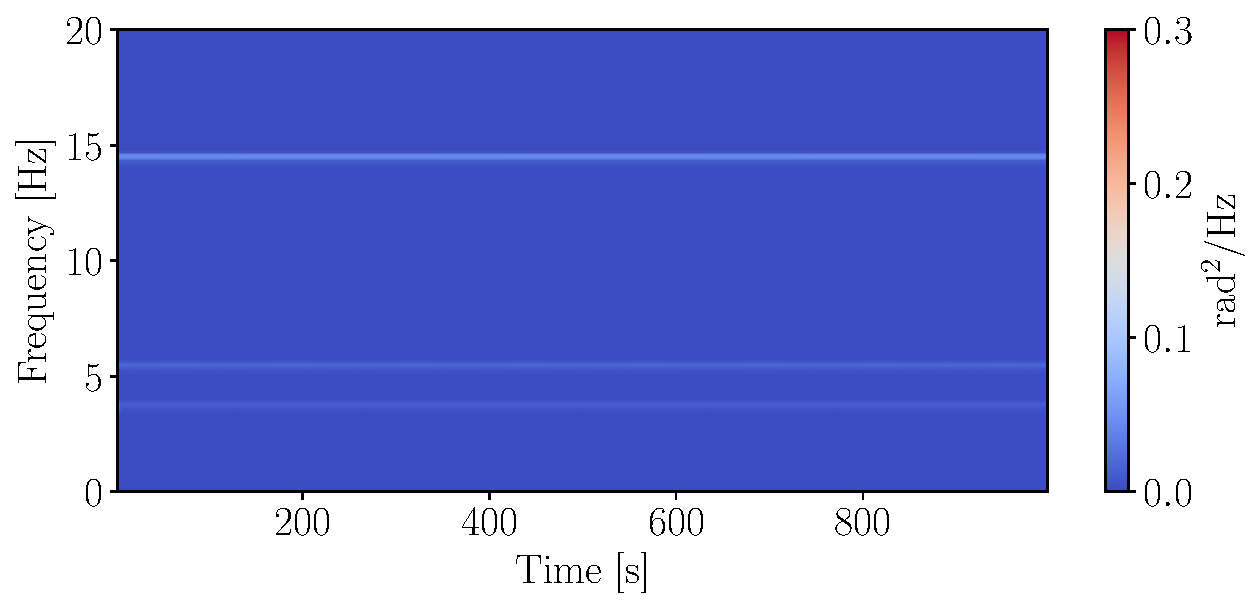
\includegraphics[width=\linewidth]{figures/plots/eadrc_ebmflc_amplitude_0.0/spectrogram_response_eadrc_ebmflc_amplitude_0.0.pdf}
      \end{minipage}

      \vspace{0.2cm}
      \begin{minipage}{0.49\linewidth}
        \centering
        {\scriptsize Sem controle, movimento}\\
        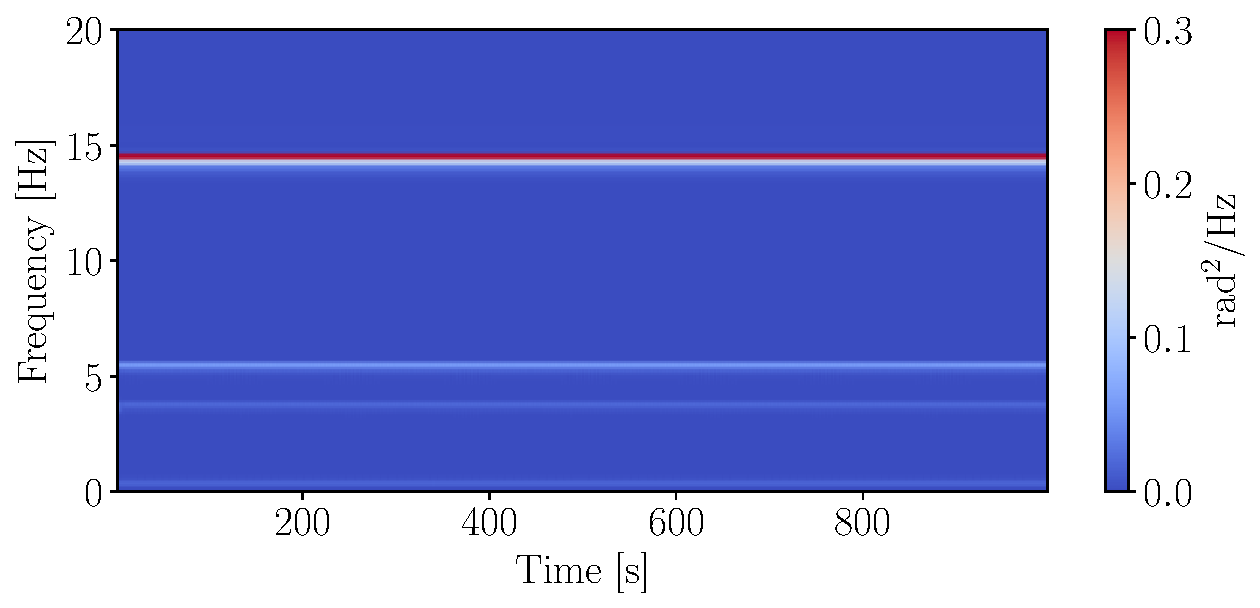
\includegraphics[width=\linewidth]{figures/plots/uncontrolled_amplitude_1.0/spectrogram_response_uncontrolled_amplitude_1.0.pdf}
      \end{minipage}
      \hfill
      \begin{minipage}{0.49\linewidth}
        \centering
        {\scriptsize EADRC+EBMFLC, movimento}\\
        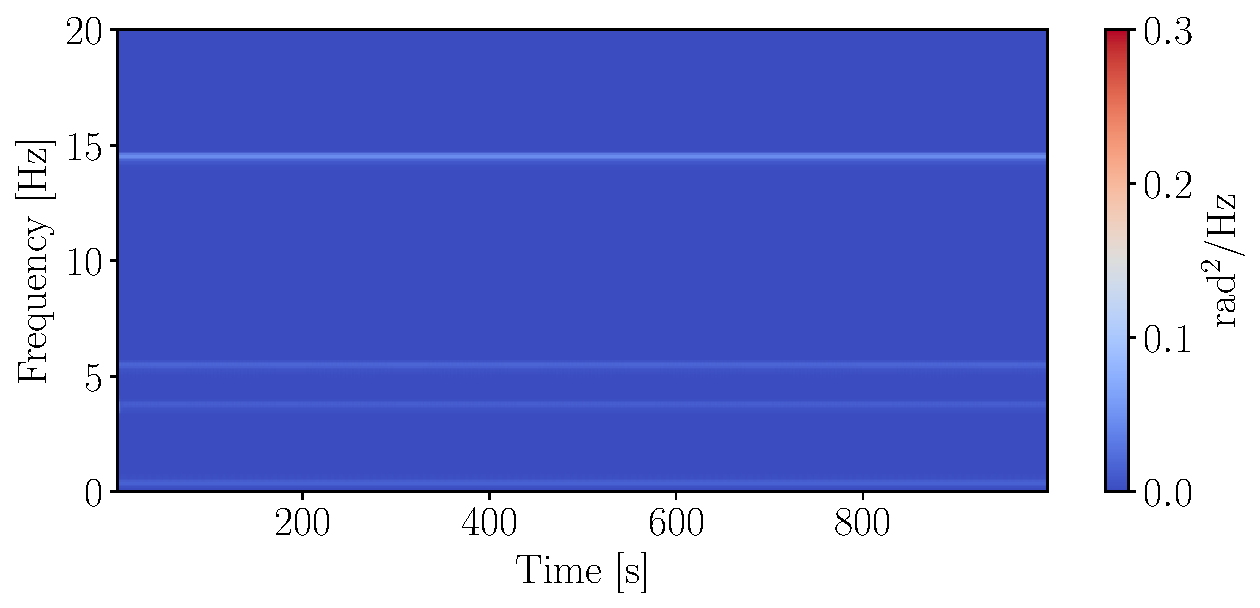
\includegraphics[width=\linewidth]{figures/plots/eadrc_ebmflc_amplitude_1.0/spectrogram_response_eadrc_ebmflc_amplitude_1.0.pdf}
      \end{minipage}

      \vspace{0.1cm}
      {\tiny Espectrogramas de simulações longas (cerca de 1000 s), para maior resolução em frequência.}
    \end{column}
    \begin{column}{0.30\textwidth}
      \small
      \begin{itemize}
        \setlength{\itemsep}{0.2cm}
        \item Componente de 14,35 Hz fortemente atenuada.
        \item Componentes de 3,59 e 5,30 Hz \alert{pouco mitigadas}.
        \item Comportamento semelhante em repouso e em movimento.
      \end{itemize}
    \end{column}
  \end{columns}
\end{frame}


\section{Conclusões}

\begin{frame}{Conclusões e trabalhos futuros}
  \begin{itemize}[<+->]
    \setlength{\itemsep}{0.1cm}
    \item EADRC para supressão do tremor de punho na DP, considerando a dinâmica acoplada do membro superior (modelo de 3 GdL).
    \item Alta supressão com menor esforço de controle que o DE-PID; entre as variantes EADRC, o ZPLP gerou sinais de controle mais suaves.
    \item EADRC+ZPLP: TPSR médio de 61,31\% em movimento, superior aos controladores clássicos realizáveis.
    \item Desempenho consistente com variações de até 50\% em rigidez e amortecimento: adequado quando as propriedades biomecânicas são incertas ou variantes no tempo.
    \item A estimação do movimento voluntário é decisiva para não deixar tremores de menor frequência fora da perturbação total estimada.
  \end{itemize}

  \pause
  \vspace{0.2cm}
  \begin{exampleblock}{Trabalhos futuros}
    Outras estratégias de controle da literatura, métodos alternativos de estimação do movimento voluntário e outros modelos do membro superior.
  \end{exampleblock}
\end{frame}


% --- Slide Final ---
\begin{frame}[plain]{Agradecimentos}
  \centering
  Agradecemos o apoio financeiro da \textbf{FAPDF} e do\\
  \textbf{Programa de Formação de Recursos Humanos da ANP}.

  {\scriptsize FAPDF nº 435/2023, Processo nº~00193-00002143/2023-02, Chamada Pública 01/2023 -- BIO Learning.}

  
\includegraphics[height=1.4cm]{fapdf.jpg}
  \hspace{0.5cm}
  
\includegraphics[height=1.2cm]{PRH-57.png}

  {\tikzset{visible on/.style = {}}\resizebox{.5\linewidth}{!}{% Workflow of the proposal, shown in "Proposta deste trabalho" and repeated in "Agradecimentos"
% (needs TikZ libraries positioning, calc and fit, the CBA colors from cba2026.sty and the
% `visible on` overlay style from presentation.tex; set \tikzset{visible on/.style={}}
% before \input to show everything at once)
\begin{tikzpicture}[
    > = latex,
    font = \small,
    node distance = 0.35cm,
    item/.style = {
        draw,
        thick,
        rounded corners = 2pt,
        align = center,
        text width = 4.1cm,
        minimum height = 1.15cm,
        inner sep = 3pt,
        execute at begin node = {\hyphenpenalty = 10000\exhyphenpenalty = 10000},
    },
    platform/.style = {item, draw = CBAOrange, fill = CBALightOrange},
    estimator/.style = {item, draw = CBAPetrol, fill = CBALightPetrol},
    control/.style = {item, draw = CBAPurple, fill = CBALightPurple},
    baseline/.style = {item, draw = CBAGraphite!60, fill = CBAGraphite!5, dashed},
    evaluation/.style = {item, draw = CBAMagenta, fill = CBALightMagenta},
    lane/.style = {
        draw = #1,
        very thick,
        rounded corners = 5pt,
        inner xsep = 0.2cm,
        inner ysep = 0.25cm,
    },
    lane title/.style = {font = \small\bfseries, text = #1, anchor = south, inner sep = 2pt},
    stage/.style = {->, line width = 2.5pt, CBAGraphite!45, shorten > = 2pt, shorten < = 2pt},
]
    % Wrist control (middle lane), centered on y = 0; the gaps leave room for the annotated arrows
    \node [control, visible on = <2->] (eadrc) at (6.1, 0)
        {EADRC no punho: rejeita a perturbação total, inclusive o acoplamento \cite{Guo:2016}};
    \node [estimator, above = 0.75cm of eadrc, visible on = <2->] (estimator)
        {Estimação de $\theta_{v_3}$: EBMFLC \cite{Atashzar:2016} ou ZPLP};
    \node [baseline, below = 0.75cm of eadrc, visible on = <2->] (baselines)
        {Comparação: IMC-PID e DE-PID ($\theta_{v_3}$ conhecido)};

    % Test platform (left lane), centered on the middle lane
    \node [platform, above = 0.2cm, visible on = <1->] (model) at (0, 0)
        {Modelo linear do membro superior com 3 GdL \cite{Gebai:2017,Gebai:2018}};
    \node [platform, below = 0.2cm, visible on = <1->] (torques) at (0, 0)
        {Torques de tremor (3 harmônicos) e voluntário (repouso ou movimento)};

    % Evaluation (right lane), centered on the middle lane
    \node [evaluation, above = 0.4cm, visible on = <3->] (monte carlo) at (12.2, 0)
        {Monte Carlo: 100 execuções pareadas em 2 cenários};
    \node [evaluation, below = 0.4cm, visible on = <3->] (statistics) at (12.2, 0)
        {6 métricas, Wilcoxon pareado e Holm-Bonferroni};

    % Lanes, each fitted to its own boxes
    \node [lane = CBAOrange, fit = (model) (torques), visible on = <1->] (platform lane) {};
    \node [lane = CBAPurple, fit = (estimator) (baselines), visible on = <2->] (control lane) {};
    \node [lane = CBAMagenta, fit = (monte carlo) (statistics), visible on = <3->] (evaluation lane) {};
    \node [lane title = CBAOrange, visible on = <1->] at (platform lane.north) {Plataforma de teste};
    \node [lane title = CBAPurple, visible on = <2->] at (control lane.north) {Controle do punho};
    \node [lane title = CBAMagenta, visible on = <3->] at (evaluation lane.north) {Avaliação};

    % Flow inside and between lanes
    \draw [->, thick, CBAPetrol, visible on = <2->] (estimator) -- (eadrc)
        node [midway, right, font = \footnotesize] {$\hat{\theta}_{v_3}$};
    \draw [thick, dashed, CBAGraphite!60, visible on = <2->] (eadrc) -- (baselines)
        node [midway, right, font = \footnotesize, text = CBAGraphite] {vs.};
    \draw [->, thick, CBAMagenta, visible on = <3->] (monte carlo) -- (statistics);
    \draw [stage, visible on = <2->] (platform lane) -- (control lane);
    \draw [stage, visible on = <3->] (control lane) -- (evaluation lane);
\end{tikzpicture}%
}}

  \textbf{Muito Obrigado!}

  {\small Contato: thiagotomasdepaula@gmail.com}

  {\small Código: https://github.com/Thiago-TP/eadrc-parkinson-suppression}
\end{frame}

% --- Material de apoio ---
\appendix
% Material de apoio (after \appendix): methods first, then statistics, then results

\begin{frame}{EBMFLC: estimação do movimento voluntário}
  \begin{columns}[T]
    \begin{column}{0.47\textwidth}
      \footnotesize
      \begin{itemize}
        \setlength{\itemsep}{0.12cm}
        \item Combinador linear de Fourier com banda limitada e memória em janela \cite{Atashzar:2016,Qi:2024}: $\theta_3$ é aproximado por $n = 100$ senoides de frequências fixas $f_r \in [0, 12]$~Hz (passo de $\approx 0{,}12$~Hz).
        \item A cada passo $k$, com $\mathbf{x}_k = [\sin\omega_r t_k \,\,\, \cos\omega_r t_k]_{r=1}^{n}$:
          \begin{equation*}
            \varepsilon_k = \theta_{3,k} - \mathbf{w}_k^\top\mathbf{x}_k,
            \quad
            \mathbf{w}_{k+1} = p\,\mathbf{w}_k + 2\mu\,\varepsilon_k\,\mathbf{x}_k.
          \end{equation*}
        \item Esquecimento $p = \alpha^{1/(f_s T_p)} \approx 0{,}9934$: uma amostra com $T_p = 0{,}59$~s de idade pesa $\alpha = 2\%$. Ainda, $\mu = 0{,}005$ e $f_s = 1$~kHz.
        \item Movimento voluntário: só os termos de até 4~Hz,
          \begin{equation*}
            \hat{\theta}_{v_3,k} = \textstyle\sum_{f_r \leq 4\,\text{Hz}} \left( w_{r}\sin\omega_r t_k + w_{n+r}\cos\omega_r t_k \right).
          \end{equation*}
      \end{itemize}
    \end{column}
    \begin{column}{0.51\textwidth}
      \centering
      \begin{tikzpicture}[
          > = latex,
          font = \footnotesize,
          block/.style = {draw, thick, rounded corners = 2pt, align = center, inner sep = 3pt, minimum height = 0.75cm},
          estimator/.style = {block, draw = CBAPetrol, fill = CBALightPetrol},
          junction/.style = {draw, thick, circle, minimum size = 0.4cm, inner sep = 0pt},
        ]
        % Adaptive loop
        \node [estimator] (reference) at (0, 0) {Senoides\\$\mathbf{x}_k$};
        \node [estimator] (combiner) at (2.3, 0) {$\mathbf{w}_k^\top\mathbf{x}_k$};
        \node [junction] (sum) at (4.3, 0) {};
        \node [estimator] (selection) at (2.3, 1.35) {Termos com $f_r \leq 4$~Hz};
        \node [estimator] (lms) at (2.3, -1.35) {LMS com esquecimento};
        \draw [->, thick] (reference) -- (combiner);
        \draw [->, thick] (combiner) -- (sum) node [pos = 0.8, above] {$-$};
        \draw [<-, thick] (sum) -- ++(1, 0) node [right] {$\theta_3$} node [pos = 0.35, above] {$+$};
        \draw [->, thick] (sum) |- (lms) node [pos = 0.3, right] {$\varepsilon_k$};
        \draw [->, thick] (reference) |- (lms);
        \draw [->, thick] (lms) -- (combiner) node [midway, right] {$\mathbf{w}_{k+1}$};
        \draw [->, thick] (combiner) -- (selection);
        \draw [->, thick, CBAPetrol] (selection) -- ++(2.4, 0) node [right] {$\hat{\theta}_{v_3}$};

        % Frequency comb of the references, split at 4 Hz
        \begin{scope}[shift = {(-0.6, -3.55)}, x = 0.37cm, y = 1cm]
          \foreach \r in {0, ..., 99} {
            \pgfmathsetmacro{\f}{12 * \r / 99}
            \pgfmathparse{\f <= 4 ? "CBAPetrol" : "CBAGraphite!35"}
            \draw [\pgfmathresult, line width = 0.6pt] (\f, 0) -- (\f, 0.5);
          }
          \draw [->, thick] (0, 0) -- (13, 0) node [right] {$f$ [Hz]};
          \foreach \f in {0, 4, 8, 12} \draw (\f, 0) -- (\f, -0.08) node [below] {\f};
          \node [above, text = CBAPetrol] at (1.6, 0.5) {voluntário};
          \node [above, text = CBAGraphite] at (8, 0.5) {tremor};
          % Tremor harmonics
          \foreach \f/\label in {3.59/{3,59}, 5.30/{5,30}} {
            \draw [CBAMagenta, thick, dashed] (\f, 0) -- (\f, 0.9) node [above, font = \scriptsize, text = CBAMagenta] {\label};
          }
          \node [right, font = \scriptsize, text = CBAMagenta, align = left] at (12.3, 0.65) {14,35 Hz:\\fora da banda};
        \end{scope}
      \end{tikzpicture}

      \vspace{0.1cm}
      {\scriptsize Tracejado: harmônicos do tremor; o de 3,59~Hz cai na banda voluntária.}
    \end{column}
  \end{columns}
\end{frame}

\begin{frame}{Hiperparâmetros dos controladores}
  \centering
  \footnotesize
\begin{tabularx}{\textwidth}{l >{\raggedright\arraybackslash}X l}
    \toprule
    Controlador & Parâmetros & Sintonia (modelo nominal) \\
    \midrule
    EADRC+ZPLP &
        $\omega_c = 10$, $\omega_o = 100$; Butterworth de 1ª ordem, corte em 5 Hz &
        Experimental, $\omega_o = 10\,\omega_c$ \\
    EADRC+EBMFLC &
        $\omega_c = 20$, $\omega_o = 80$; $n = 100$, $\mu = 0{,}005$, $T_p = 0{,}59$~s, $\alpha = 0{,}02$ &
        Experimental, $\omega_o = 4\,\omega_c$ \\
    IMC-PID &
        $K_p = 1{,}235$, $K_i = 1234{,}660$, $K_d = 0{,}506$ &
        IMC \cite{Rivera:1986}, punho isolado, $\lambda = 0{,}4\,\tau$ \\
    DE-PID &
        $K_p = 1{,}721$, $K_i = 15{,}059$, $K_d = 3{,}239$ &
        Evolução diferencial, $\theta_{v_3}$ conhecido \\
    \bottomrule
\end{tabularx}


  \vspace{0.3cm}
  \raggedright
  \footnotesize
  \begin{itemize}
    \setlength{\itemsep}{0.1cm}
    \item EADRC parametrizado por largura de banda: ESO com $\beta_1 = 3\omega_o$, $\beta_2 = 3\omega_o^2$, $\beta_3 = \omega_o^3$; lei PD com $\kappa_1 = \omega_c^2$, $\kappa_2 = 2\omega_c$; $b_0 = [\mathbf{J}^{-1}]_{33}$.
    \item PIDs discretos com passo $\Delta t = 1$~ms: $u_{3,k} = K_p e_k + K_i \sum_{j \leq k} e_j \Delta t + K_d (e_k - e_{k-1}) / \Delta t$; o IMC-PID estima $\theta_{v_3}$ com o mesmo filtro do ZPLP.
    \item Todos sintonizados no modelo nominal e mantidos fixos nas 100 execuções.
  \end{itemize}
\end{frame}

\begin{frame}{Sintonia do IMC-PID}
  \begin{columns}[T]
    \begin{column}{0.53\textwidth}
      \footnotesize
      \begin{itemize}
        \setlength{\itemsep}{0.12cm}
        \item Modelo de projeto: punho isolado, sem o acoplamento com ombro e cotovelo,
          \begin{equation*}
            G(s) = \frac{1}{J_{33}s^2 + c_4 s + k_4} = \frac{K}{\tau^2 s^2 + 2\zeta\tau s + 1}.
          \end{equation*}
        \item IMC \cite{Rivera:1986}: $Q(s) = G^{-1}(s)\,\frac{1}{\lambda s + 1}$, de modo que a malha nominal é $\frac{1}{\lambda s + 1}$. O controlador clássico equivalente é um PID ideal:
          \begin{gather*}
            C(s) = \frac{Q}{1 - GQ} = \frac{\tau^2 s^2 + 2\zeta\tau s + 1}{K\lambda s}, \\
            K_p = \frac{2\zeta\tau}{K\lambda}, \quad
            K_i = \frac{K_p}{2\zeta\tau}, \quad
            K_d = \frac{K_p\,\tau}{2\zeta}.
          \end{gather*}
        \item Velocidade da malha: $\lambda = f\,\tau$, com $f$ escolhido por busca em grade, $f \in \{0{,}1;\, 0{,}2;\, \dots;\, 5{,}0\}$, maximizando $R^2$ no modelo nominal em movimento.
      \end{itemize}
    \end{column}
    \begin{column}{0.45\textwidth}
      \begin{block}{Valores (modelo nominal)}
        \footnotesize
        \begin{itemize}
          \item $J_{33} = 0{,}0041$~kg$\cdot$m$^2$, $k_4 = 10$~N$\cdot$m/rad, $c_4 = 0{,}01$~N$\cdot$m$\cdot$s/rad.
          \item $K = 1/k_4$, $\tau = \sqrt{J_{33}/k_4} = 0{,}0202$~s e $\zeta = c_4 / (2\sqrt{J_{33}k_4}) = 0{,}0247$: polos complexos, pouco amortecidos.
          \item Melhor $f = 0{,}4$ nos dois cenários, logo $\lambda = 0{,}0081$~s: $K_p = 1{,}235$, $K_i = 1234{,}7$ e $K_d = 0{,}506$.
        \end{itemize}
      \end{block}
      \begin{alertblock}{Limitação}
        \footnotesize
        O modelo ignora o acoplamento, e a malha rápida ($\lambda < \tau$) não tolera bem a incerteza: em 4 (repouso) e 5 (movimento) das 99 execuções perturbadas, a oscilação cresce.
      \end{alertblock}
    \end{column}
  \end{columns}
\end{frame}

\begin{frame}{Sintonia do DE-PID por evolução diferencial}
  \begin{columns}[T]
    \begin{column}{0.53\textwidth}
      \footnotesize
      Busca de $\mathbf{x} = (K_p, K_i, K_d) \in [0, 5] \times [0, 100] \times [0, 5]$ que minimiza $J(\mathbf{x}) = -R^2$ no modelo nominal, com rastreamento perfeito ($\hat{\theta}_{v_3} = \theta_{v_3}$); simulações instáveis recebem $J = 10^{12}$.

      \vspace{0.15cm}
      DE/best/1/bin \cite{Storn:1997}, a cada geração e para cada indivíduo $\mathbf{x}_i$:
      \begin{enumerate}
        \setlength{\itemsep}{0.08cm}
        \item \alert{Mutação}: $\mathbf{v} = \mathbf{x}_{\text{best}} + F\,(\mathbf{x}_{r_1} - \mathbf{x}_{r_2})$, com $r_1 \neq r_2$ sorteados e $F \sim \mathcal{U}(0{,}5;\, 1)$ por geração.
        \item \alert{Cruzamento binomial}: $u_j = v_j$ se $\mathcal{U}(0, 1) < CR = 0{,}7$ ou $j = j_{\text{rand}}$; senão, $u_j = x_{i,j}$.
        \item \alert{Seleção}: $\mathbf{x}_i \leftarrow \mathbf{u}$ se $J(\mathbf{u}) \leq J(\mathbf{x}_i)$, atualizando o melhor imediatamente.
      \end{enumerate}
    \end{column}
    \begin{column}{0.45\textwidth}
      \begin{block}{Configuração e resultado}
        \footnotesize
        \begin{itemize}
          \item População de 15 indivíduos ($5 \times 3$ ganhos), iniciada por hipercubo latino; semente 42; sem polimento local.
          \item Parada: 30 gerações ou $\sigma(J) \leq 10^{-3}\,|\overline{J}|$ na população; convergiu na 8ª geração, com 135 simulações.
          \item $K_p = 1{,}721$, $K_i = 15{,}059$ e $K_d = 3{,}239$ nos dois cenários, com $R^2 \approx 0{,}999$.
        \end{itemize}
      \end{block}
      \vspace{0.1cm}
      {\tiny Implementação: \texttt{scipy.optimize.differential\_evolution}, em \texttt{src/pid\_tuning.py}.}
    \end{column}
  \end{columns}
\end{frame}

\begin{frame}{Teste de postos sinalizados de Wilcoxon}
  \begin{columns}[T]
    \begin{column}{0.55\textwidth}
      \footnotesize
      Por cenário, métrica $M$ e controlador de comparação, com a mesma rigidez na execução $j$ (amostras pareadas), $d_j = M_j^{\text{ZPLP}} - M_j^{\text{outro}}$, $j = 1, \dots, 100$.
      $H_0$: distribuição de $d$ simétrica em torno de 0, bilateral \cite{Wilcoxon:1945,Conover:1980}.
      \begin{enumerate}
        \setlength{\itemsep}{0.05cm}
        \item \alert{Zeros} ($d_j = 0$) são descartados; $n$ é o número de $d_j \neq 0$.
        \item Postos de $|d_j|$; \alert{empates} recebem o posto médio.
        \item $R^{+}$ e $R^{-}$: somas dos postos de $d_j > 0$ e de $d_j < 0$.
        \item Aproximação normal, com correção de continuidade e de empates ($t_g$: tamanho do grupo $g$ de empates):
          \begin{gather*}
            \mu = \tfrac{n(n+1)}{4},
            \quad
            \sigma^2 = \tfrac{n(n+1)(2n+1)}{24} - \textstyle\sum_g \tfrac{t_g^3 - t_g}{48}, \\
            z = \frac{R^{+} - \mu - \frac{1}{2}\operatorname{sgn}(R^{+} - \mu)}{\sigma},
            \quad
            p = 2\left[1 - \Phi(|z|)\right].
          \end{gather*}
        \item Tamanho de efeito: $r = (R^{+} - R^{-}) / (R^{+} + R^{-}) \in [-1, 1]$ \cite{Kerby:2014}.
      \end{enumerate}
    \end{column}
    \begin{column}{0.43\textwidth}
      \begin{block}{Nos dados}
        \footnotesize
        \begin{itemize}
          \item $n = 100$ nos 36 testes: \alert{nenhum zero e nenhum empate}, pois as métricas são contínuas.
          \item $|r| = 1$ quando uma estratégia vence em todas as execuções: $\min(R^{+}, R^{-}) = 0$, $|z| = 8{,}68$ e $p = 3{,}96 \cdot 10^{-18}$, o menor $p$ possível com $n = 100$.
        \end{itemize}
      \end{block}
      \begin{exampleblock}{Implementação}
        \footnotesize
        \raggedright
        \texttt{scipy.stats.wilcoxon} (SciPy 1.18.1), com \texttt{zero\_method="wilcox"}, \texttt{correction=True} e aproximação normal. Reproduzido à mão, com erro relativo em $p$ abaixo de $10^{-13}$.
      \end{exampleblock}
    \end{column}
  \end{columns}
\end{frame}

\begin{frame}{Correção de Holm-Bonferroni}
  \begin{columns}[T]
    \begin{column}{0.45\textwidth}
      \footnotesize
      \begin{itemize}
        \setlength{\itemsep}{0.15cm}
        \item Por cenário, $m = 18$ testes (6 métricas $\times$ 3 comparações). Sem correção, com $\alpha = 0{,}05$ e testes independentes, a chance de ao menos um falso positivo seria $1 - 0{,}95^{18} \approx 60\%$.
        \item Procedimento de Holm \cite{Holm:1979}: ordenam-se $p_{(1)} \leq \dots \leq p_{(m)}$ e
          \begin{equation*}
            \tilde{p}_{(k)} = \min\Big\{1, \max_{j \leq k} \,(m - j + 1)\, p_{(j)}\Big\};
          \end{equation*}
          $H_{(k)}$ é rejeitada se $\tilde{p}_{(k)} < \alpha$.
        \item Limita a taxa de erro por família a $\alpha$ sob qualquer dependência entre os testes e nunca é menos poderoso que Bonferroni ($m\,p_{(k)}$); o máximo acumulado mantém $\tilde{p}$ monótono.
      \end{itemize}
    \end{column}
    \begin{column}{0.53\textwidth}
      \centering
      {\small Exemplo: repouso}

      \vspace{0.1cm}
      \scriptsize
      \setlength{\tabcolsep}{2.5pt}
      \begin{tabular}{r l c c c}
        \toprule
        $k$ & ZPLP vs. & $p_{(k)}$ & $m - k + 1$ & $\tilde{p}_{(k)}$ \\
        \midrule
        1  & DE-PID, TPSR      & $3{,}96 \cdot 10^{-18}$ & 18 & $7{,}12 \cdot 10^{-17}$ \\
        \multicolumn{5}{c}{$\vdots$} \\
        9  & DE-PID, entropia  & $5{,}19 \cdot 10^{-18}$ & 10 & $7{,}12 \cdot 10^{-17}$\textsuperscript{*} \\
        10 & IMC-PID, TPSR     & $3{,}23 \cdot 10^{-16}$ & 9  & $2{,}91 \cdot 10^{-15}$ \\
        11 & IMC-PID, $R^2$    & $3{,}42 \cdot 10^{-16}$ & 8  & $2{,}91 \cdot 10^{-15}$\textsuperscript{**} \\
        \multicolumn{5}{c}{$\vdots$} \\
        17 & EBMFLC, TPSR      & $1{,}35 \cdot 10^{-6}$  & 2  & $2{,}70 \cdot 10^{-6}$ \\
        18 & EBMFLC, entropia  & $0{,}365$               & 1  & \alert{$0{,}365$} \\
        \bottomrule
      \end{tabular}

      \vspace{0.15cm}
      \raggedright
      Máximo acumulado: \textsuperscript{*}$10\,p_{(9)} = 5{,}2 \cdot 10^{-17}$, mas vale o de $k = 1$; \textsuperscript{**}$8\,p_{(11)} = 2{,}74 \cdot 10^{-15}$, mas vale o de $k = 10$.
      Em vermelho, o único teste não significativo do cenário.

      \vspace{0.2cm}
      \structure{Implementação:} \texttt{holm\_bonferroni()}, em \texttt{statistics.py}, com uma família de 18 testes por cenário.

    \end{column}
  \end{columns}
\end{frame}

\begin{frame}{Respostas temporais no modelo nominal}
  \centering
  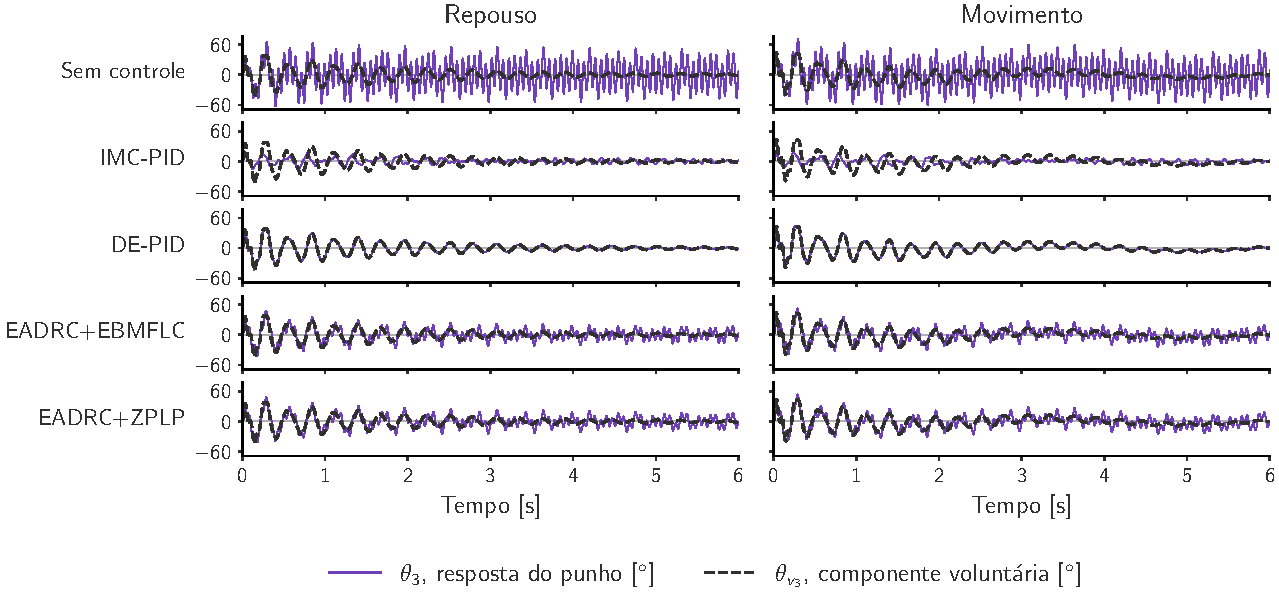
\includegraphics[width=\linewidth,height=0.9\textheight,keepaspectratio]{time_responses.pdf}
\end{frame}

\begin{frame}[allowframebreaks]{Referências}
  \printbibliography
\end{frame}


\end{document}
